\section{Design}

\begin{figure}
\centering
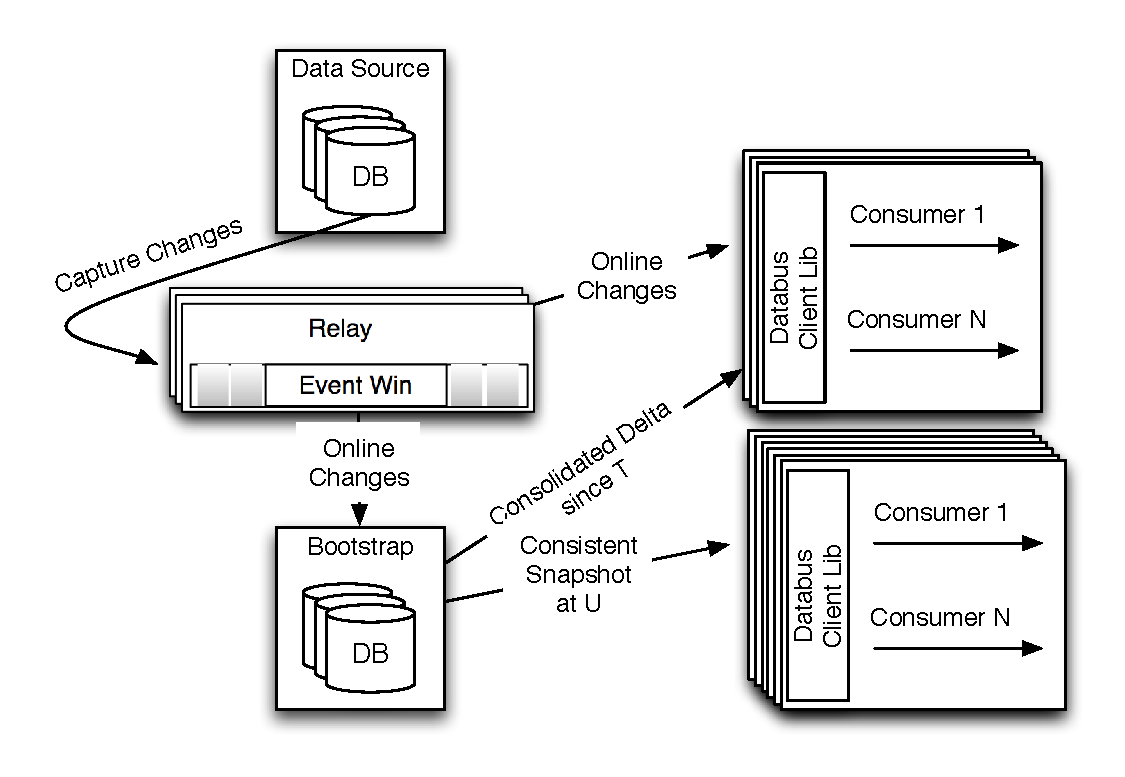
\epsfig{file=figures/databus-arch.eps, width=3.2in}
\caption{Databus Architecture}
\label{fig:databus-architecture}
\end{figure}

The Databus transport system is split into four logical parts. 
\begin{itemize}
\item a \emph{fetcher} which extracts changes from the source, 
\item a \emph{log store} which caches this change stream, 
\item a \emph{snapshot store} which stores a moving snapshot of the stream, and 
\item a \emph{subscription client} which moves seamlessly between the various components to provide changes to the application. 
\end{itemize}

The typical deployment architecture for these modules is shown in Figure~\ref{fig:databus-architecture}. We collocate the fetcher and an in-memory log store in a process we call the \emph{relay} process. We additionally collocate a persistent log store and the snapshot store in a process we call the \emph{bootstrap server}. The subscription client is a library that is linked into the application that needs to consume changes from the stream. For a new type of data source, the only component that needs to change in this architecture is the implementation of the fetcher. 
 
\subsection{Semantics}
Databus supports transactional semantics across multiple types of entities within a transactional datastore. For example, it can annotate and propagate transactions that span multiple tables within the same database. It supports guaranteed at-least once delivery semantics by default. A single event is delivered multiple times only in the case of failures in the communication channel between the relay and the client, or in case of a hard failure in the consumer application. A consumer which keeps exact checkpoints even across failures can perform de-duping to get exactly once delivery. The guarantee of lossless delivery is provided by the end-to-end pull architecture in Databus. Every failure can be recovered from by going up the chain and re-pulling from the checkpoint of the failure point. 

\subsection{The Fetcher: External Clock and Pull model}

The design philosophy of Databus is that it is simply a transporter of changes that have been committed upstream. Each change or change-set is expected to be annotated with a monotonically increasing clock value which we refer to as the SCN of the change or change-set. As changes flow throughout the data architecture, derived state gets created by applications and needs to be associated back to the change stream that generated that state. This is important not just for auditing, but also to recover from failures and resume processing without missing any changes. 
The entire Databus infrastructure therefore tracks the lineage of data records and the progress of consumers using only the clock of the external system. Physical offsets in transport are only used as optimizations but are never used as source of truth. This is a very important design decision because it allows an application to bootstrap itself with a snapshot of data that it might have procured outside the Databus ecosystem. For example, an application can take a dump of an Oracle database, perform arbitrary processing on that dump, and then seamlessly tap into the Databus stream to get all changes that have happened to the database without missing a single change. The only requirement is that the original Oracle dump should be stamped with the same clock that the Oracle Databus fetcher uses to pull changes out from Oracle. Figure~\ref{fig:pull-model} shows the interactions between the different fetcher components and the source clock across the relay, bootstrap log and snapshot store. In this example, the source has generated changes until sequence number 102400, the relay has an in-memory buffer that covers all changes from 70000 to 100000, the bootstrap server's persistent log covers all changes from 30000 to 90000, and the bootstrap server's snapshot store covers all changes from 0 to 80000. Depending on where the consumer is currently at, it will pull from either the relay or the bootstrap server. 

\begin{figure}
\centering
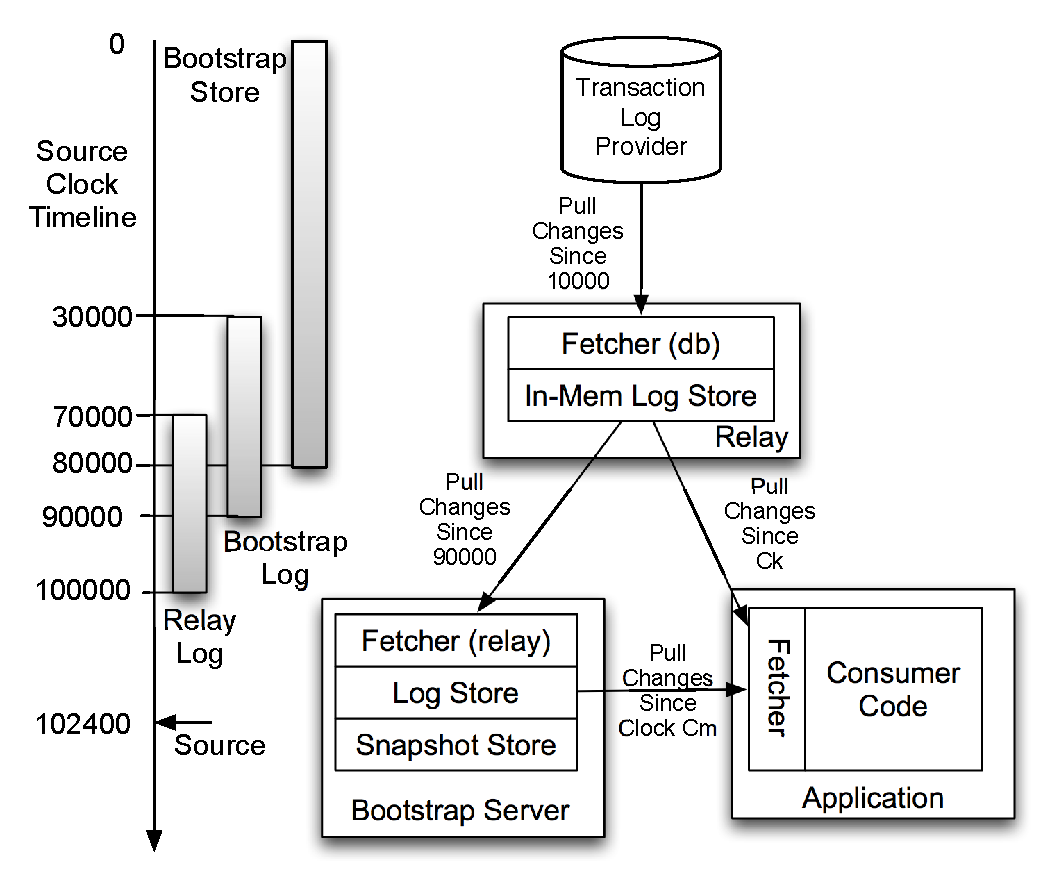
\epsfig{file=figures/databus-pull-model.eps, scale=0.50}
\caption{Pull Model and Source Clock}
\label{fig:pull-model}
\end{figure}

Fetchers keep track of where they are in the timeline using checkpoints which typically contain a highwatermark corresponding to the contiguous section of the timeline that has been reliably processed so far. The fetcher is expected to be initialized with a checkpoint when it starts up or recovers from a failure. Once initialized, the fetcher keeps pulling changes from the data-source from that checkpoint onwards. As changes get processed, the fetcher keeps advancing the highwatermark and periodically stores the checkpoint in some persistence layer. This pure pull model ensures that the Databus transport layer is lossless. The only guarantees needed from the persistence layer is to not lose changes out of order. Similarly, the only requirement this adds on the data source is that it should be able to support rewindable consumption; the fetcher can sometimes go back in time on failures. In most of the systems we've seen, this requirement does not add extra complexity on the source as long as this lookback window is bounded (within a day or two). The way the Oracle fetcher is written, it can go back all the way to time zero, but at the cost of queries that get progressively expensive. The MySQL fetcher can rewind back to as much time as the storage on the MySQL machine will allow to retain, without any performance penalties. This centralization of complexity onto the fetcher component leads to very simple persistence and failure-recovery protocols downstream.

\subsection{The Relay}
The Databus relay hosts a fetcher, a transient log and an HTTP server within a single process. The fetcher is a pluggable entity and can be used to fetch changes from a source or from another relay. The pluggability allows us to customize the change extractor for a specific datasource.

The change extractor serializes the changes to a data source independent
binary format. These changes are grouped together by transaction window boundaries and are annotated with the clock id associated with the transaction. 
\begin{figure}
\centering
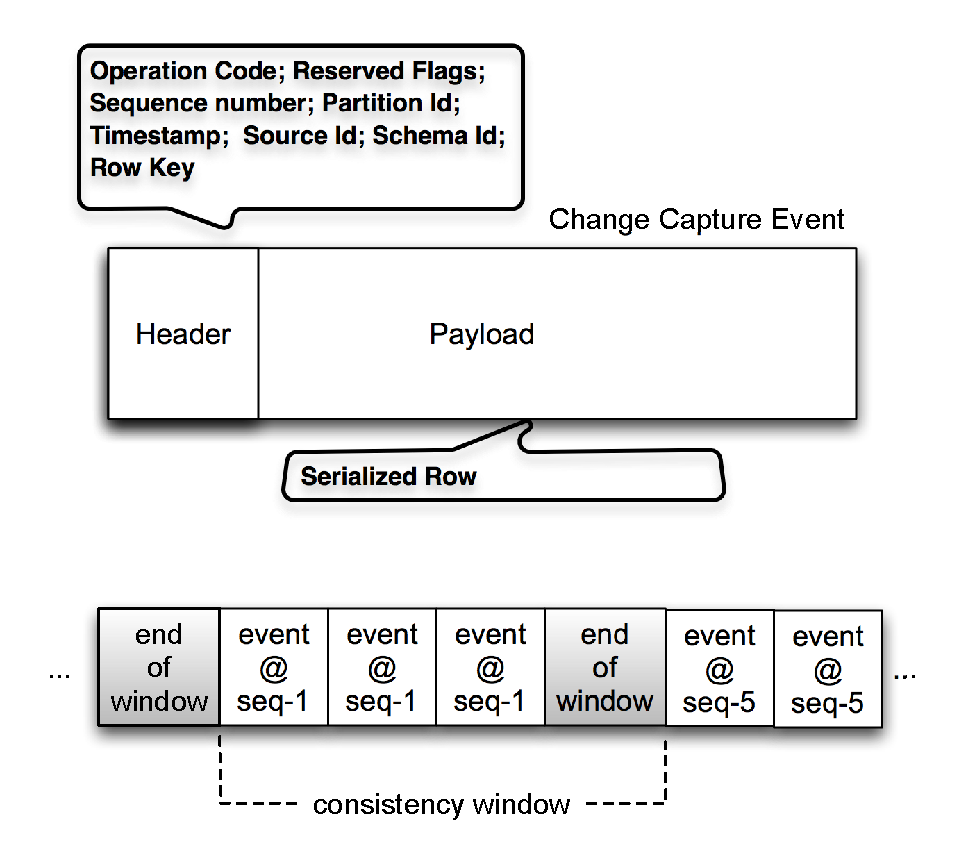
\epsfig{file=figures/change-capture-format.eps, width=3in}
\caption{Change Capture Window Format}
\label{fig:change-capture-window-format}
\end{figure}
Figure~\ref{fig:change-capture-window-format} shows the organization of a single transaction window.
The serialized changes are stored in the log which is used to serve the changes to the clients. 
\begin{figure}
\centering
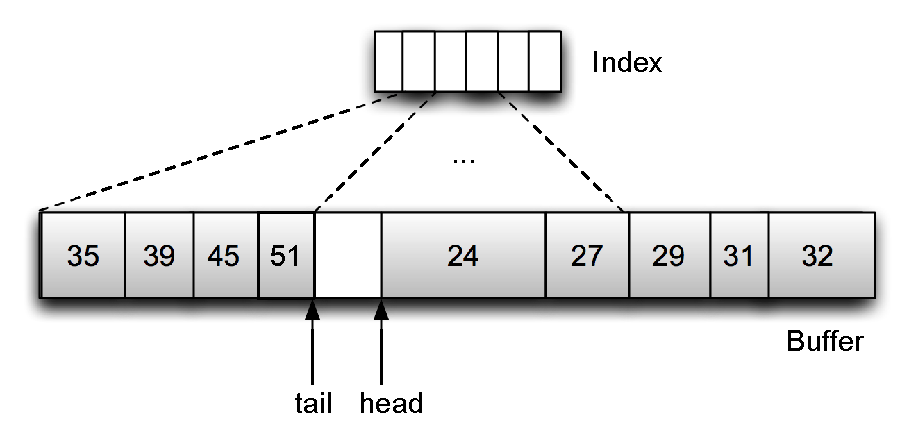
\epsfig{file=figures/relay-data-structures.eps, width=3.2in}
\caption{Buffer and Index Data Structures}
\label{fig:buffer-index}
\end{figure}
Figure~\ref{fig:buffer-index} shows the data structures used to implement the log. We made some interesting design decisions while implementing the log. 
\begin{itemize}
\item \emph{Off-heap}: Processes that allocate large amounts of long-lived memory inside the Java Virtual Machine (JVM) tend to suffer from garbage collection related performance issues. In fact, the original implementation of the Databus relay log had this problem. We therefore decided to keep the buffer allocated outside the JVM heap. 
\item \emph{Space-bound}: With multi-tenancy in mind, we wanted to support setting limits on how much space the buffer could use. This naturally led us to build it as a circular buffer with the changes pre-serialized and inline. This supports very fast insert performance and also naturally supports range scans. There is no new memory allocated after the relay starts up, which leads to very stable and predictable performance.
\item \emph{Indexed}: Since the range scans are based on an external clock, we also need an index to speed up the scans. To do this, we use another bounded circular buffer which functions as a skip-list on top of the buffer. Thus the total amount of memory that a particular log needs is always bounded. We trade-off some scan latency for space in this case. 
\item \emph{Concurrent}: The circular design forces us to consider writes and readers potentially stepping on each others toes. Simple reader-writer locks create too much contention and limit throughput unnecessarily. Region-based locking increases throughput somewhat but still penalizes the common case when readers are caught up with the writer. In this case, there is one hot region at the tail end of the buffer where writes are happening after the tail, and reads are happening just before the tail. Using range-based locking in this case solves this problem quite elegantly, and ensures maximal read-write throughput for non-colliding reads and writes. In practice, we hardly see any contention in real workloads because readers and writers are pretty much in lock-step most of the time. However when the readers start falling behind, their range lock eventually conflicts with the writer's range lock, and then get evicted off the relay. 
\item \emph{Filtering}: We support server-side filtering by brute-force scanning the changes and streaming out only the events that match the subscriber's filter pattern. For mmapped buffers, we avoid double-copying between user-space and file-system, and yet retain the ability to filter out data when we stream it out.
\end{itemize}

An important point to note is that the relay is a stateless service and does not track where consumers are in the timeline. This simplifies the relay's implementation but requires a time or size-based retention policy. In practice, we over-provision the relay to keep multiple days worth of buffer which is enough to ensure that all the caught-up and online consumers can consume the whole stream while just consuming from the relay. Using mmapped buffers allows us to provision more than the amount of available physical memory on the relay node. The predictable pattern of sequential read and write along with the locality of access (writer is always writing at the tail, readers are typically very close to the tail) means that only the most recent pages need to be in memory.  

\begin{algorithm}
\label{alg:stream-call}{stream}{($checkpoint$, $sources$, $filters$, $maxBytes$, $channel$)}
\caption{Databus Relay Stream Algorithm}
\begin{algorithmic}
\STATE Consult index to determine the start of the scan
\STATE Acquire read range lock from scanOffset to tail
%%\STATE $scanOffset \leftarrow index$.getOffset($checkpoint$)
\FOR{$event$ in $range$($scanOffset$, tail)}
\IF{the $event$ matches the $filters$ and we have not exceeded $maxBytes$}
%%$filters$.match($event$) and $sizeNotExceeded$}
\STATE write $event$ to the $channel$
%%$channel$.write($event$)
%%\STATE $checkpoint$.apply($event$)
\ENDIF
\ENDFOR
%%\STATE $channel$.write($checkpoint$.toString())
\STATE write $endOfStreamMarker$ to the $channel$
%%$channel$.write($endOfStreamMarker$)
\end{algorithmic}
\end{algorithm} 

The pseudo-code for the primary stream call is documented at Algorithm~\ref{alg:stream-call}. The primary input parameters into this call are the consumer's checkpoint, the list of tables they are interested in and any subscription filters that they want to apply additionally on the changes. The stream call first determines the scan offset to begin the scan, then acquires a read range lock from the offset to the tail of the buffer. It then iterates through the buffer streaming out any events that match the filter. The stopping condition is either reaching the end of the buffer or hitting the maximum size limit set by the consumer. 




\subsection{The Bootstrap Service}
\label{subsec:Bootstrap}

As we have described previously, consumers typically subscribe to changes from the relay, which maintains an in-memory log store. Occasionally, there are situations in which the consumers might fall significantly behind in their processing. This usually happens because of consumer failures, which cause them to be offline for an extended period of time. In other cases, new consumers are launched and they need to bootstrap their initial state before consuming the change log from the relay. 

Possible approaches for dealing with these situations are going back to the source OLTP database and storing extended logs at the relays. The first approach is not acceptable since it leads to greatly increased load on the database that is serving online traffic. Besides, getting a consistent snapshot of all the rows in the OLTP database by running a long running query is very difficult. Storing the log at the relay for extended periods of time is not always viable since if the consumer has fallen behind a lot, consuming every change event is likely to be slow and unnecessary. It is much more efficient to catch up using a snapshot store which is a compacted representation of the changes i.e. only the latest state of every affected row needs to be consumed. 

Databus implements this functionality using a Bootstrap Service. As shown in Figure~\ref{fig:databus-architecture}, the bootstrap service consists of three components:
\begin{itemize*}
\item a \emph{bootstrap database}: This has two parts. One is a persistent log store that maintains the change log for an extended time. The other is a snapshot store of the data that represents a view of the database at a given point in time. 
\item a \emph{bootstrap producer}: This is really just a fetcher that subscribes to the change log from the relay and writes it to the log store in the bootstrap database. 
\item and a \emph{bootstrap applier}: This is just another fetcher that pulls from the log store and periodically merges the changes into the snapshot.
\end{itemize*}

%Splitting the responsibilities between the bootstrap producer and the bootstrap applier  has two advantages. First, it keeps the change log persistent over an extended period of time so that consumers that fall behind and do not find changes on the relay can catch up using the log in the bootstrap database. Second, it is able to handle long transactions on the source OLTP database easily since appending to the log is much cheaper than building the snapshot. This ensures that the bootstrap database has enough write throughput to keep up with the source. 

In the above design, the combination of both a snapshot store and a log store is what ensures the ability of the Bootstrap Service to provide consistent snapshots to the consumer applications from arbitrary points in the change stream. It is important to note that the snapshot store itself is not sufficient to achieve this goal as explained below.

Getting a consistent read of the snapshot by locking the snapshot store is not practical. For big data sets, it may take many hours for a consumer application to read and process the snapshot. If there are multiple consumers trying to bootstrap, the application of new changes to the snapshot store may be suspended indefinitely. Further, if the entire snapshot is read in one humongous batch, a small processing error may require restarting of the entire bootstrapping process. Instead, the Bootstrap Service needs to allow the consumer application to bootstrap the data in manageable batch sizes while new changes are applied to the snapshot store. Thus at the end of reading the snapshot, it may not be consistent -- the consumer application may have been observed some of the new changes while it may have missed others. To ensure consistency, the Bootstrap Service has to replay all the changes that have happened from the point when the snapshot read started. Thus, the need for a log store to buffer such changes.

Further, splitting the responsibilities between the relay fetcher and the log store fetcher ensures that the Bootstrap Service has enough write throughput to keep up with the data source: appending to the log store is much cheaper than building the snapshot store. Peaks in the write traffic are handled gracefully by letting the snapshot store lag slightly behind the newest changes.

The full bootstrapping algorithm with support for bootstrapping of multiple sources is described below.

%On the consumer side, when a consumer needs to bootstrap, it needs to obtain the change events from both the snapshot and log store so that the combination yields a consistent change set. This is complicated by the fact that the bootstrap producer is updating the snapshot simultaneously. Getting a consistent read of the snapshot by locking the snapshot is not efficient when it is large. Instead the consumer must constantly be allowed to make progress by pulling rows in manageable batch sizes while applier is merging changes from the log store. Since the snapshot data might change across batches, this results in an inconsistent read of the data during the time rows are being read from the snapshot store.  In order to guarantee consistent read at the end of the bootstrapping phase,  bootstrap service uses the following algorithm to deliver changes to the consumer.

\begin{algorithm}
\label{alg:bootstrap}
\caption{Bootstrap Consumption}{bootstrap}{($sources$)} 
\begin{algorithmic}
\STATE $startScn$ = current scn of the bootstrap db
\FOR{$i=0$ to $sources$.length}
\REQUIRE Source $S_{j}$ ($j < i$) is consistent as of $startScn$ \\
\COMMENT{Begin Snapshot phase}
\STATE Get all rows from $S_{i}$ where $rowScn < startScn$ \\
\COMMENT{Can be done in batches}
\STATE $targetScn$ = max SCN of rows in $S_{i}$
\COMMENT{Begin Catchup phase}
\FORALL{source $S$j such that $j \leq i$}
\STATE Get all rows from $S_{j}$ log store from startScn until targetScn
\ENDFOR
\STATE $startScn = targetScn$
\ENDFOR
\end{algorithmic}
\end{algorithm}

\subsection{Event Model and Consumer API}

\lstset{basicstyle=\small}


There are two versions of the consumer API, one that is callback driven and another that is iterator-based. 
At a high-level, there are eight main methods on the Databus callback API.
%%We show the callback based API at Listing~\ref{listing:DatabusConsumerAPI}.   
%%\begin{algorithm}
%%\lstset{caption={Databus Consumer API},label=listing:DatabusConsumerAPI}
%%\begin{lstlisting}
%%interface DatabusEventListener
%%{
%%  Result onStartDataEventSequence(SCN startScn);
%% Result onEndDataEventSequence(SCN endScn);
%% Result onStartSource(String source, 
%%                       Schema srcSchema);
%%  Result onEndSource(String source, 
%%                     Schema srcSchema);
%%  Result onDataEvent(DbusEvent e, 
%%                     DbusEventDecoder decoder);
%%  Result onCheckpoint(SCN checkpointScn);
%%  Result onRollback(SCN rollbackScn);
%%  Result onError(SCN rollbackScn);
%%}
%%\end{lstlisting}
%%\end{algorithm}

\begin{itemize*}
\item \emph{onStartDataEventSequence}: the start of a sequence of data events from an events consistency window.
\item \emph{onStartSource}: the start of data events from the same Databus source (e.g. Oracle table). 
\item \emph{onDataEvent}: a data change event for the current Databus source.
\item \emph{onEndSource}: the end of data change events from the same Databus source.
\item \emph{onEndDataEventSequence}: the end of a sequence of data events with the same SCN.
\item \emph{onCheckpoint}: a hint from the Databus client library that it wants to mark the point in the stream identified by the SCN as a recovery point
\item \emph{onRollback}: Databus has detected a recoverable error while processing the current event consistency window and it will rollback to the last successful checkpoint.
\item \emph{onError}: Databus has detected a unrecoverable error and it will stop processing the event stream.
\end{itemize*}.

The above callbacks denote the important points in the stream of Databus change events. A typical sequence of callbacks follows the pattern below.

\begin{verbatim}
onStartDataEventSequence(startSCN)
    onStartSource(Table1)
        onDataEvent(Table1.event1)
               ...
        onDataEvent(Table1.eventN) 
    onEndSource(Table1)
    onStartSource(Table2)
        onDataEvent(Table2.event1) 
              ...
        onDataEvent(Table2.eventM)
    onEndSource(Table2)
        ... 
onEndDataEventSequence(endSCN)
\end{verbatim}

Intuitively, the Databus client communicates with the consumer: "Here is the next batch of changes in the watched tables (sources). The changes are broken down by tables. Here are the changes in the first table, then the changes to the next table, etc. All the changes represent the delta from the previous consistent state of the database to the following consistent state."

The contract on all of the callbacks is that the processing code can return a result code denoting a successful processing of the callback, recoverable or unrecoverable error. Failures to process the callback within the allocated time budget or throwing an exception, results in a recoverable error.
In cases of recoverable errors, the client library will rollback to the last successful checkpoint and replay the callbacks from that point.

The offloading of state-keeping responsibility from the consumer simplifies the consumer recovery. The consumer or a newly spawned consumer can rewind back to the last known good checkpoint. For instance, if the consumer is stateful, they just need to tie the state that they are keeping with the checkpoint of the stream. On failure, the new consumer can read the state and the checkpoint associated with it and just start consuming from that point. If the stream consumption is idempotent, then the checkpoint can be maintained lazily as well. 


\subsection{Metadata} 
\begin{figure*}
\centering
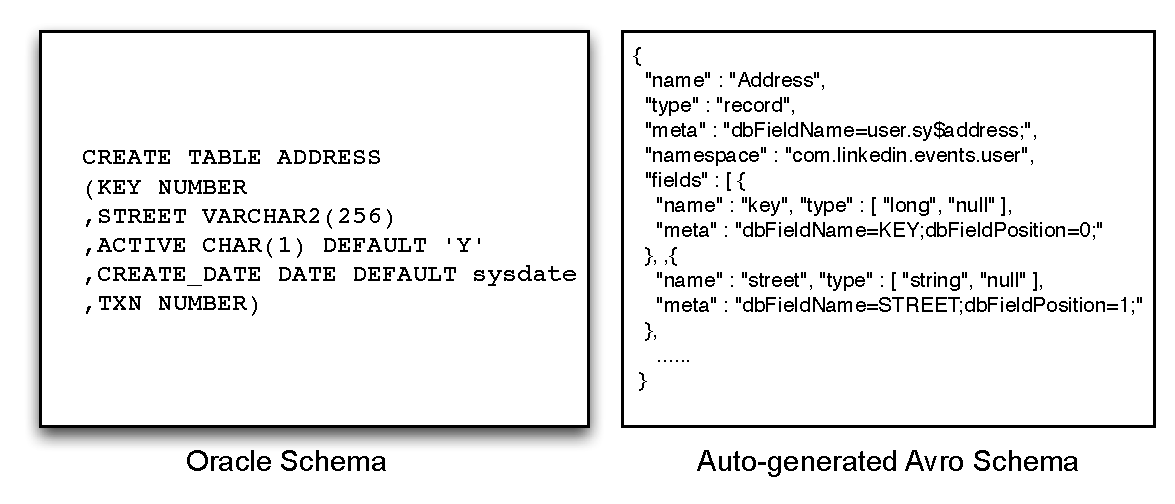
\epsfig{file=figures/oracle-avro-schema.eps, scale=0.75}
\caption{Oracle table mapped to Avro schema}
\label{fig:schema-mapping}
\end{figure*}

Databus uses Avro for serialization of events and supports schema versioning and evolution. This provides an isolation layer that protects consumers from upstream changes in the schema.

The fetchers infer the Avro schema by inspecting the source tables. Figure~\ref{fig:schema-mapping} shows a simple Oracle table mapped to an Avro schema. There are some intricacies when mapping data-types, e.g. when you have a column defined as NUMBER in Oracle, which one of int, long, float do you use when referring to the column in Avro? Once a schema is inferred, the relay is notified about it. When the fetcher generates new events from this table, it serializes the events with the Avro schema. When a table evolves, the schema for it changes and Databus attaches a newer version identifier to it. All new events are now serialized with this new schema version identifier. 

Databus ensures that changes to the source schema do not affect consumers and they can upgrade at their own cadence. The Databus client library performs automatic schema conversion using the standard  Avro schema resolution rules~\cite{avro} . We do not require reserialization of all older events generated since the beginning of time when the schema evolves because all versions of the schema are kept around forever. The schema resolution to an older version of the event schema is performed dynamically at the callback to the consumer. 

\subsubsection{Relay Cluster Deployment}

Typical Databus deployments consist of a cluster of relay servers that pull change streams from multiple data sources. Each relay server can connect to multiple data source servers and host the change stream from each server in separate buffers in the same relay. The relays are also set up in such a way that the change stream from every data source is available in multiple relays, for fault-tolerance and for consumer scaling. There are two configurations the relays are typically deployed.

\begin{figure}
\centering
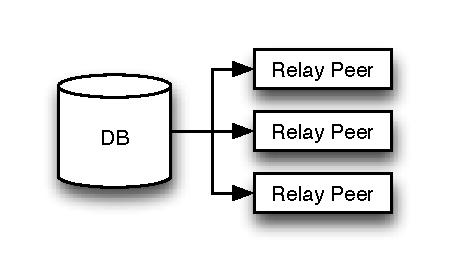
\epsfig{file=figures/relay_deployment_peers.eps, width=2.5in}
\caption{Independent Relay Deployment}
\label{fig:RelayDeployment1}
\end{figure}

In one deployment model as shown in Figure~\ref{fig:RelayDeployment1}, all the relay servers hosting a stream connect to the stream's data source directly. Each relay server is assigned a subset of all the streams being hosted by the relay cluster. The relay connects to the specified data source server and pulls the change streams. When a relay fails, the surviving relays continue pulling the change streams independent of the failed relay. If the configured redundancy factor is R, this model provides 100\% availability of the streams at very low latency as long as all the R relays that connect to the same data source server do not fail at the same time. This however comes as the cost of increased load on the data source server since there are R relays that pull the same change stream.

\begin{figure}
\centering
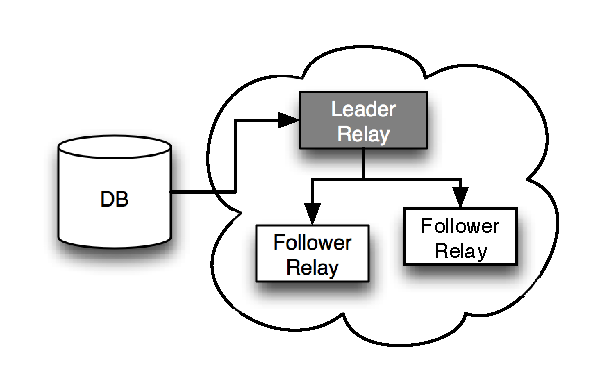
\epsfig{file=figures/relay_deployment_leader.eps, width=3in}
\caption{Leader-Follower Relay Deployment}
\label{fig:RelayDeployment2}
\end{figure}

To reduce the load on the source data source server, an alternative deployment model for relays as shown in Figure~\ref{fig:RelayDeployment2}, is the Leader-Follower model. In this model, for every data source server, one relay is designated to be the leader while R-1 are designated to be followers. The leader relay connects to the data source to pull the change stream while the follower relays pull the change stream from the leader. The clients can connect to any of the relays, either leader or follower. If the leader relay fails, one of the surviving followers is elected to be the new leader. The new leader connects to the data source server and continues pulling the change stream from the last sequence number it has. The followers disconnect from the failed leader and connect to the new leader. This deployment drastically reduces the load on the data source server but when the leader fails, there is a small delay while a new leader is elected. During this window, the latest changes in the change stream from the data source server are not available to the consumers.

To expand the capacity of the relay cluster, new relay servers can be added. When this happens, a new assignment of data source servers to relay servers is generated so that some streams are transferred from the old relay servers to the new relay servers. The new relay servers then connect to the data source servers and start pulling the change streams. They can optionally copy the existing change streams from the old relay servers before connecting to the data source servers.
This management of the relay cluster is built on top of a generic cluster management framework built at LinkedIn called Helix.

The assignment of data sources to relays is made available to Databus consumers in the form of a routing table so that the clients can discover the location of the streams they wish to consume. When the assignment changes due to relay failures or relay cluster rebalancing, this routing table is automatically updated and the consumers switch to the new servers transparently.


